\section{Introduction}

% MARKER: ho detto che i materiali vanno caratterizzati con la resistenza media?
% MARKER: guidelines/standards invece che altra roba

% MARKER: citare che NZSEE permette di usare ASCE 41 o EC8 a patto di calcolare NBS

The assessment of the seismic performance of existing buildings is a complex process since, typically, those are not specifically designed to resist earthquakes. With respect to new structures, more advanced and detailed modelling, analysis and verification procedures are needed, since existing buildings are not specifically designed to exclude a priori the formation of unfavourable, local and global failure mechanisms, which may be difficult to analyse.

The understanding of the structural behaviour of structures under seismic attack has significantly evolved in the last decades, starting in the 1970s with the concept of capacity design, introduced in New Zealand, \cite{hollings1969}, and finally developed in a pioneering book by \cite{park1975}. Considering the high expansion of the cities in the second half of the XX century, it can be stated that a considerable number of the existing buildings was designed having little or no consideration of the seismic actions.

Also the realisation of the existence of a large portfolio of structures subjected to high seismic risk evolved with time, with a step-change in the 1980s, after several human lives and economic losses caused by major earthquakes around the world (e.g. 1989 Loma Prieta, USA, 1995 Kobe, Japan, 1999 Izmit, Turkey, among others).

Clearly, great research effort was sustained in earthquake-risk areas in the world (USA, New Zealand, Japan, Europe) aiming to give recommendations and/or provisions for the assessment of existing structures. For this reason, the best seismic assessment standards/guidelines are written in these regions.

In this Chapter, the assessment standards/guidelines applied in USA, Europe and New Zealand at the time of this thesis work are discussed and compared both in terms of basic principles and suggested analysis techniques. It is worth noting that the European standards are almost entirely implemented in the Italian standards, with minor modifications. The Japanese standards are not included, considering the difficulty in finding up-to-date documents in english language.

Finally, a critical comparison of the considered guidelines/standards is drawn to highlight both good practices and improvable aspects of the selected approaches.


\section{Basic principles of the considered codes}

The guidelines/standards for seismic assessment in USA, Europe and New Zealand are compared in terms of general principles, considered limit states, allowed analysis methods, safety verifications and suggested models for the calculation of the capacity of the members. The analysis methods are described in more detail in Section \ref{codes:methods}.


\subsection{ASCE 41- 13}

The USA standards document \cite{ASCE41}, \textit{Seismic Evaluation and Retrofit of Existing Buildings} (Figure \ref{fig:ASCEcover}) is the result of the update and combination of \cite{ASCE31} related to seismic assessment procedures and \cite{ASCE41-06} related to retrofit interventions. This document is comprehensive of all technical advances in the field collected in the recent years up to 2013.

\begin{figure}[h]
\begin{center}
    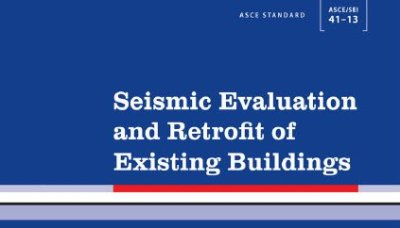
\includegraphics[width=1\textwidth]{./CHAP1/img/ASCEcover}
\caption{Seismic Evaluation and Retrofit of Existing Buildings (cover), modified after \cite{ASCE41}.}
\label{fig:ASCEcover}
\end{center}
\end{figure}


\begin{table}[!h] %MARKER: posizione tabella
\footnotesize
\centering
\caption{Criteria to qualify for the different knowledge levels.}
\label{tab:EC8criteria}
\begin{tabular}{cccccc}
\toprule
\begin{tabular}[c]{@{}l@{}}Knowledge\\ Level\end{tabular} & Geometry                                                                                                                                          & Details                                                                                                                                                                          & Materials                                                                                                                                                  & CF                                                     \\ \midrule
KL1                                                       & \begin{tabular}[c]{@{}l@{}}From original\\ outline\\ construction\\ drawings with\\ sample visual\\ survey\\ or\\ from full\\ survey\end{tabular} & \begin{tabular}[c]{@{}l@{}}Simulated design in\\ accordance with\\ relevant practice\\ and,from limited in-situ\\ inspection\end{tabular}                                        & \begin{tabular}[c]{@{}l@{}}Default values in\\ accordance with\\ standards of the\\ time of construction\\ and from limited\\ in-situ testing\end{tabular} & \begin{tabular}[c]{@{}l@{}}$CF_{KL1}$\\ (1.35)\end{tabular} \\
KL2                                                       & as for KL1                                                                                                                                        & \begin{tabular}[c]{@{}l@{}}From incomplete\\ original detailed\\ construction drawings\\ with limited in-situ\\ inspection\\ or from extended in-\\ situ inspection\end{tabular} & \begin{tabular}[c]{@{}l@{}}From original\\ design\\ specifications with\\ limited in-situ\\ testing\\ or from extended\\ in-situ testing\end{tabular}      & \begin{tabular}[c]{@{}l@{}}$CF_{KL2}$\\ (1.2)\end{tabular}  \\
KL3                                                       & as for KL1                                                                                                                                        & \begin{tabular}[c]{@{}l@{}}From original detailed\\ construction drawings\\ with limited in-situ\\ inspection\\ or from\\ comprehensive in-situ\\ inspection\end{tabular}        & \begin{tabular}[c]{@{}l@{}}From original test\\ reports with limited\\ in-situ testing\\ or from\\ comprehensive in-\\ situ testing\end{tabular}           & \begin{tabular}[c]{@{}l@{}}$CF_{KL3}$\\ (1.0)\end{tabular}  \\ \bottomrule
\end{tabular}
\end{table}



